\documentclass[reprint,unsortedaddress,amsmath,amssymb,aps,prl,showkeys]{revtex4-2}
\usepackage{graphicx}% Include figure files
\usepackage{dcolumn}% Align table columns on decimal point
\usepackage{subfigure}
\usepackage{bookmark}
\usepackage{float}
\usepackage{url}
\usepackage{bm}% bold math
\usepackage{hyperref}% add hypertext capabilities
\usepackage[mathlines]{lineno}% Enable numbering of text and display math

\begin{document}

\title{Vicissitudes of Cities Driven by Re-distributive Growth}
\author{Gezhi Xiu, Jianying Wang, Lei Dong}
\author{Yu Liu}
\email{liuyu@urban.pku.edu.cn}
\affiliation{Institute of Remote Sensing and Geographic Information Systems (IRSGIS), Peking University}
\date{\today}

\begin{abstract}
    Empirical evidence suggests that the evolution of urban systems is not only determined by local conditions, such as topography, industrial base, and group constitutions, but also is constrained by regional status, e.g., railway conveniences, regional industrial roles, and urban niches. These facts can be attributed to the competition for space and resource. Thus, modeling the emergence of cities needs to be conducted from a regional restrictive perspective. To account for this, we propose an out-of-equilibrium model of emerging cities in a given region with a fixed bound on systematic growth rates representing competitions. The model processes through a freely growing phase and a restricted growing phase. We find that empirical Zipf's and Clark's laws for cities exist in the first phase, but vanish in the second. Instead, given finite regional resource, the post phase of our model predicts the inevitability of various urban diseases such as urban shrinkage phenomenon in developed cities and the spatial transitions of developmental focuses. 
\end{abstract}
\maketitle
\section{Introduction}

% 研究的是一个什么问题(spatial growth model),这个问题为什么重要?(可以从理论和实践两个角度说,但偏重于理论)
The rapid urbanization in the past few decades brings an utmost importance of the
interdisciplinary urban studies from a complex systems perspective. Elaborately, many spatial growth models have been shown the effectiveness in explaining urban phenomena, such as urban scaling laws\cite{court2013origins}, fractality\cite{batty1994fractal,batty2007cities}, and city size distributions\cite{zipf1949human}. Furthermore, these models give quantitative predictions broadly to urban morphology and spatial structures\cite{anas1998urban}. 
% 现在的研究做了什么(现在这块写得太宽泛了,其实相关工作很多,也很具体),有哪些不足?这些不足产生的「可能的」原因是什么?

Existing works have gained insights underlying the complex features of cities, especially those developing cities in population and their spatial sprawls. The macroscopic urban aspects, e.g., the size distributions, are usually presented by multiplicative or correlated percolation\cite{makse1995modelling,PhysRevE.58.7054,rybski2013distance} models. Their formations, including the spatial explicit preferential attachment\cite{schweitzer1998estimation}, or resource utilization\cite{PhysRevE.90.042815} mechanisms which leads to the proportional growth of each cities, result in a Zipfian distribution of city rank size. On other hand, the economies of scale provided city-wise, represented by urban scaling laws\cite{court2013origins,batty2019urbanscalinglaw,bettencourt2007growth}, are realized through the characterization of human interactions, especially spatial networks\cite{marsili1998interacting,court2013origins,Li2017Simple}. These depictions have widely crossed human actions\cite{ccolak2016understanding,louf2014congestion,fujita1976spatial}. These models function in specific spatial scale under certain equilibrium conditions in growth rates or optimization aims\cite{zipf1949human}. However, urban systems are dynamic, and necessarily out-of-equilibrium with limitations in economical, political, topographical, and many other sustainability goals that lead to vicissitudinary
development\cite{parris2003characterizing,batty2008size}. For instance, city’s attractiveness is not eternal as its marginal effect for latter stage of urbanization\cite{atkinson2012urban,girardin2009quantifying}. Meanwhile, the present spatial growth models still lack the ability to capture the competition among cities in both space and resource. To address this issue needs a cross-scale consideration of inter- and intra-city formation in growth dynamics, and some sustainable conditions.

% 我们是怎么来解决这个问题的,有哪些重要的贡献。


%These concerns call for a general approach to model the spatial sprawl of emerging cities and their population under sustainable rules, regarding the competitions for space and resource.
Here, we propose an out-of-equilibrium spatial preferential growth model with restrictions on the maximum systematic rate to grow. In some non-spatial context\cite{PhysRevE.55.R3817}, a finite population has been proved to put severe constraints on the patterns of  evolution, which can be specified as urban rank-size distribution here. This restriction is proved later to enhance the intensity of competitions, resulting in realistic urban phenomena like dual cities\cite{silverman2018rethinking}, superior switch\cite{gabaix2004evolution}, and urban shrinkage\cite{haase2014conceptualizing}, that cannot be formulated by existing growth models. The spatial aspect of our model takes the idea of diffusion-limited aggregation\cite{makse1995modelling, rybski2013distance}. In other words, new comers would settle near those active citizens, to be involved in the economies of scale\cite{kleinberg2000navigation}.

\section{Results}

\subsection{The Spatial Yule Model}
% 我们提出了一个模型,能干什么事儿,有什么好处。
Our model tells how cities emerge, grow, and compete over a closed region of a 2-dimensional continuous space. As this model regards the growth of cities as how active dwellers constantly introduce new citizens, its dynamics are determined through a dearth of quantitative and spatial rules. \emph{Quantitatively}, denote $k$ and $N_i$ as the number of cities and the volume of active citizens in the $i$th city, respectively. By active we mean in urban growth process, only these citizens attracts new comers to a nearby place in her city. Here, we take $\sum_{i} N_i \le N^*$ as the satiation condition, i.e., when the population of the whole region exceeds $N^*$, an introduction of new active citizen deactivates a random dweller who is previously active. This mechanism keeps only up to $N^*$ citizens registered as introducers. Therefore we say these $N^*$ people add up to the \emph{memory kernel}. Thus we define the model in terms of a two-phase master equation, assigning $N_i$ to the growth rate of a city. Namely, we assume that the probability of a population increase in city $i$ within the time interval $(t,t+dt)$ is $\beta_2N_idt$. We also assume that with a small probability proportional to the number of cities, $\beta_1kdt$, a new city is created with one citizen. The master equation can therefore be written as \begin{align}\frac{\partial}{\partial t}N_i(t) =  \delta_{N_i(t)}\cdot k\beta_1+ (1-\delta_{N_i(t)})\cdot N\beta_2, \end{align} for the free growth phase, and \begin{align}
	\frac{\partial N_i(t)}{\partial t}  = (N^*\beta_2)[\frac{N_i(t)}{N^*}\cdot(1-N_i(t)/(N^*-1))& \notag\\  - (1-N_i(t)/N^*)\cdot (1-N_i(t)/(N^*-1)) ]&
\end{align}
for the resource constraint phase. Assigning the constants $\beta_1$ and $\beta_2$ specifies the model. Competition for more active population helps us set up the constraint in systematic resource. 
\begin{figure}
	\centering
	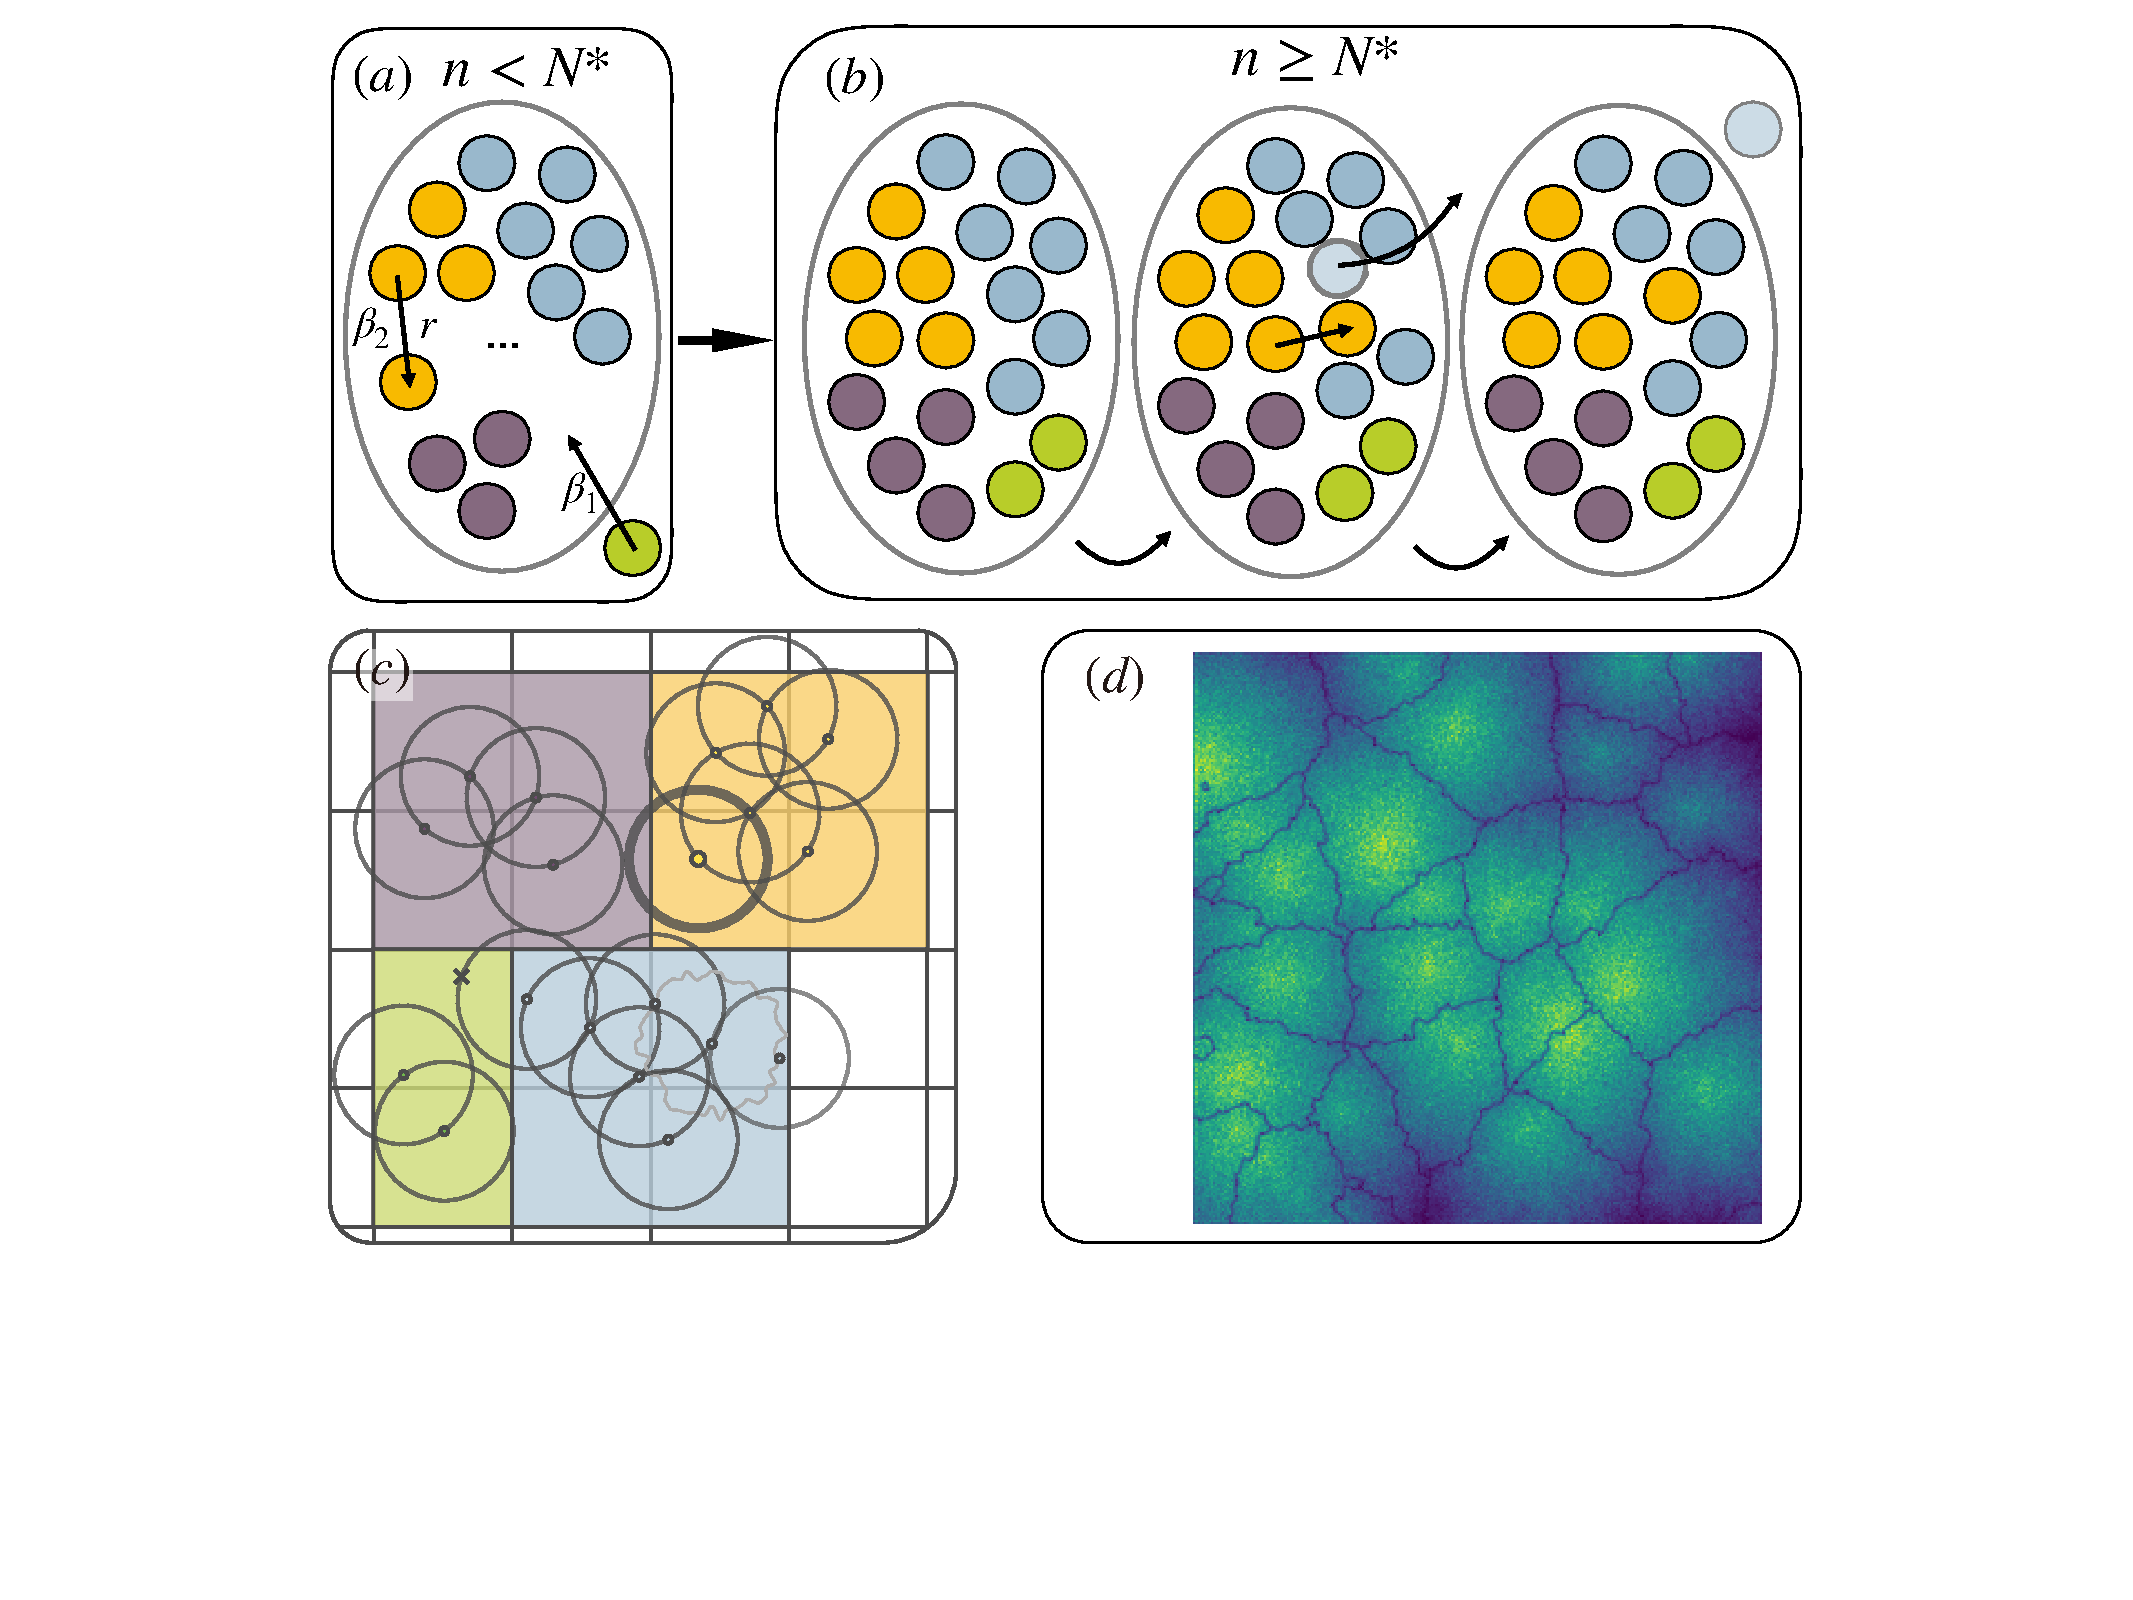
\includegraphics[width = 0.95\linewidth]{pics/sketchgood.pdf}
	\caption{(a) Status in the memory kernel at the first phase, where the total population is less than $N^*$. Existing citizens introduce new dwellers at the rate $\beta_2$, while each existing city (noted by nodes in different colors) introduces new cities at the rate $\beta_1$. (b) When the memory kernel is fulfilled, every introduction of new city or citizen leads to an ejection of existing active citizen currently included in the memory kernel. (c) The spatial aspect is that, an offspring citizen's placement is at distance $r$ from the ancestral dweller. Also, when the kernel is filled, a new yellow node ejects an existed blue node, or equivalently deprive her ability to introduce. (d) A simulated result for $L$, $r$, $\beta$ equals to $256$, $0.5$, and $4$, respectively.}
	\label{sketchpic}
\end{figure}

The \emph{spatial} growth rules consist of three parts. We first assume the studied area is an $L\times L$ grid of cells. Secondly we achieve the competition for space: Once a cell have held a citizen from the $i$th city, any citizens from another city $j$ that $j\ne i$ cannot introduce new comers on that cell; Cities are established randomly over untaken cells; Thirdly, the coordinates of citizens belong to $\mathbb{R}^2$, and every new citizen settles at a constant distance $r$ and an random angle $\theta$ from its introducer.

Since the setting of relative growth rate $\beta:= \beta_2/\beta_1$ is parallel Yule's work on the distribution of species per genus\cite{yule1925ii}, in the following text we refer our model as Spatial Yule models with constraints (SYM). A sketch for the SYM is shown in Fig. \ref{sketchpic}.

% 5. 模型需要哪些假设 6. 这些假设有什么理论和实证基础?
The SYM is based on mainly three realistic assumptions. Basically, to insure the appearance of free growth phase, the region is naturally assumed to be sufficiently large and active ($L\gg 1$, $N^*\gg 1$), while the impact of a citizen is restrained within the neighborhood($r\le 1$). Secondly but most importantly, urban developments are density driven (active citizens are attractive). Literature has suggested that density-driven social ties and interactions comprise an important driver of the economies of scale\cite{pan2013urban, girardin2009quantifying, batty1992form}. In the SYM, we further assume only the density of attractive population are corresponding to urban developments. Such active part can be recognized as the total employed or productive people. Combined with the grid structure of the SYM, we can further analyze the density dynamics both collectively and internally, leading to Zipf's law and phenomenal urban shrinkage, respectively. Thirdly, to make it analytical, we assume a homogeneous background in two parts: New cities' establishment is a Poisson point process over all untaken cells\cite{miles1970homogeneous}; And active citizens at different position introduce new comers at the same rate. This diffusive setting of sequential settlements is also realistic urban growth\cite{RevModPhys.87.925}. Meanwhile, the last setting copes with Clark's law, the exponential decay of urban population density from urban center\cite{clark1951urban}.

In the numerical experiments, we conclude that $L = 256$ is sufficiently large for the free growth phase to emerge. So the truly worth-tuning parameters are only three. $\beta$ contributes to the Zipf's coefficient and later defined turnover rate\cite{rooney2006structural}; $r$ contributes to fractality of urban envelops and the time to fill the whole space; And $N^*$ is the severeness of resource competition which results in the fluctuation of turnover rate.

% 7. 这个模型能推出哪些结论(1,2,3)。这些结论能如何被数据验证。
\subsection{The free growth phase}

Depending on the relative importance of city sprawl, emergence rate, and economic constraints, SYM predicts the existence of three phases: freely growth phase, economic constraint phase, and spatial constraint phase. We focus on the first two phases, which correspond with cities' memory. In the freely growth phase, cities grow desolately, without being controlled by total resource and space. We now describe its two important properties, stately (1) Zipf's law\cite{gabaix1999zipf's} for rank size distribution of cities' population, and (2) Clark's law for exponential decay of urban density. The validation of these laws confirm that SYM is a valid model for urban systems.

The populations of cities typically decay proportionally to the inverse of their ranks\cite{gabaix1999zipf's}. This is referred as Zipf's law of cities' population sizes, i.e., the populations of cities distribute as a power of ranks, $f_r(r)\sim r^{-(1+\beta)}$. Recall that the number of individuals in the system at time $t$, $N_i(t)$, has a geometric distribution\cite{durrett1999essentials}, $P(N_i(t)=n)=e^{-\beta_1t}(1-\exp(- {\beta_1} t))^{n-1}$, and the second assumption that the number of cities will grow exponentially at rate $k\beta_1$, if we pick a random city, the time since its first appearance waits exponential times with parameter $\beta_1$. Thus the distribution of population of a random city is 
\begin{align}
	f(n)=\frac{\Gamma(1+1/\beta)\Gamma(n)}{\beta\Gamma(n+1+1/\beta)}\approx Cn^{-1-1/\beta}, \ \text{as } n\to\infty,
\end{align}
where $\Gamma(\cdot)$ is the gamma function. This implies a Zipf's relationship with $n(\text{rank})\sim {rank}^{-\beta}$. Noticing that $\beta$ takes value from all positive real number in SYM, we can derive arbitrary scaling behaviors by switching $\beta$. According to some existing studies\cite{PhysRevLett.79.523}, the power law dependence of population frequency is $2.03\pm 0.05$ for the world, indicating the average relative emerging rate of cities is around $1.03$. 

Varying $\beta$ leads to the consideration of different sizes of study area. A small $\beta$ means the emergence of cities is fast, which corresponds to a large spatial scale. The problem of determining the relative speed of city's generation, is very reminiscent of some problems encountered in gas physics. It is interesting to investigate the number of cities in a given regions of the same population. Some groups tend to form new cities to have sufficient infrastructures and less diversity of urban output ($\beta > 1$) and some cities may go otherwise ($\beta< 1$). This value is actually a reflection of the intensity of regional industry. The experiments have confirmed our analytic results for the first phase in SYM. A simulated validation for this result can be reflected in Fig.\@\ref{fig:rankditribution}. Notably, for increasing $\beta$s, the simulated Zipfian exponents are remarkably larger than their theoretical predictions. This is because the competition for space benefits large small cities resulted from their higher density of edging cells, but large $\beta$s the probability of successful emergence of small cities drop. This exasperate the concentration of active population in large cities.
\begin{figure}[t]
	\centering
	\subfigure[Rank]{
		\begin{minipage}[t]{0.98\linewidth}
			\centering
			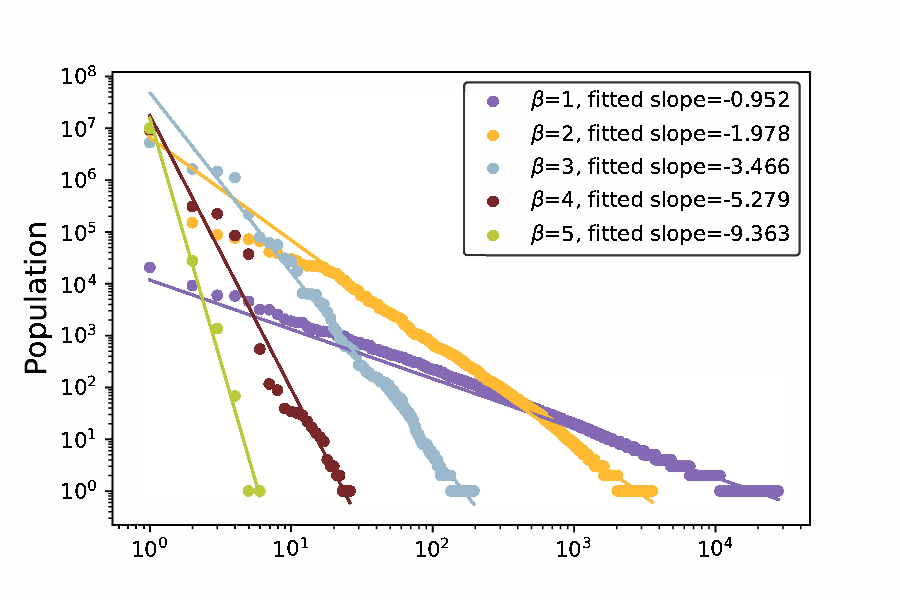
\includegraphics[width=\textwidth]{pics/zipf.pdf}
		\end{minipage}%
	\label{fig:rankditribution}
	}
	\subfigure[Distance to the urban center]{
	\begin{minipage}[t]{0.98\linewidth}
		\centering
		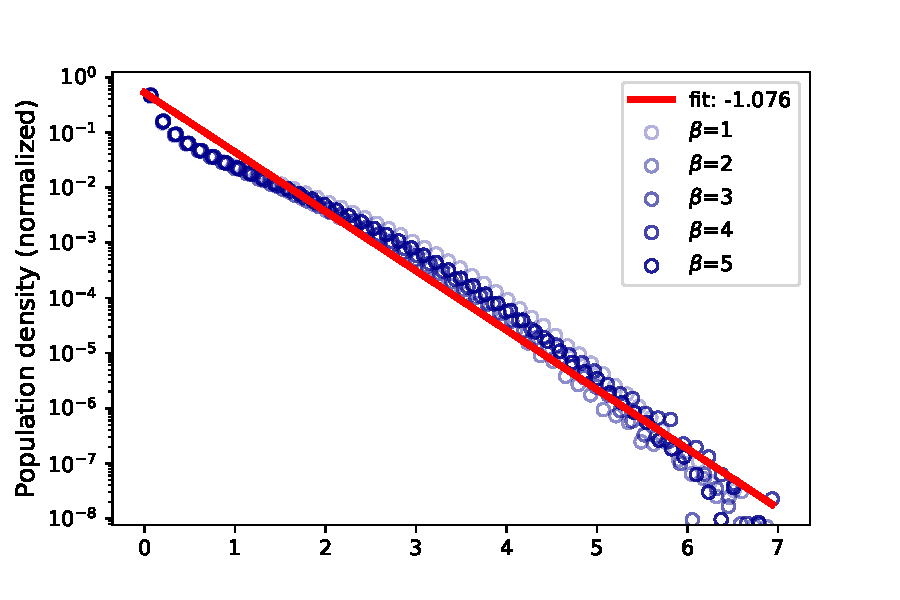
\includegraphics[width=\textwidth]{pics/kernal_density.pdf}
		\label{fig:clark}
	\end{minipage}%
}
	\caption{\textbf{(a)} The distribution of population among cities. In the simulation we take $N^* = 10^5$ and alternate $\beta$s. The realistic Zipf's coefficient is reproduced when $\beta\approx 1$. The theoretical predictions of the slopes are $-\beta$, and is well approximated when $\beta$s are small. Larger $\beta$ reduce the chance of latter city's emergence. Thus the spatial aspects of the SYM strengthen inequality. This result confirms that Zipf's law is valid for growing urban systems where all cities share the same rate to grow. From the other master equation we analyze that this observation vanishes if total growing force is finite. \textbf{(b)} The population distribution as a function of distance from a district's center. The vertical axis is logarithmic processed, which represents the exponential decaying of population distribution. Regardless of the finite-sample effect, we fit the middle part of spatial population density to the exponential distribution with a slope of $-1.076$.}
\end{figure}

%% clark

Population density evolves as two-dimensional diffusion within a city\cite{doi:10.1137/0150099}, where we can focus the density's growth on each axis from the oldest citizens of a city. Let $
(d)$ denote the active population density of locations at the distance $d$ from a city's center, and $t_n$ as the time for the $n$'th citizen to generate, we have 
\begin{align}
	\rho_{t_{n+1}}(d) = (\rho_{t_{n}}(d-r) + \rho_{t_{n}}(d+r) )/2.\label{loc_den}  
\end{align} By re-scaling time as $\tau_n = t_n\cdot (k\beta_1+N\beta_2)/T$, for a sufficient large $T$, this equation\@\ref{loc_den} results in an exponential decay of density
\begin{align}
	\rho(d)\sim e^{-\alpha d}\label{clark_eq}.
\end{align}
This is a reinvention of Clark's law in empirical urban studies\cite{clark1951urban}. Beyond solitary growth, we analyze the competitiveness of land for different cities. The population within an edging cell of city $j$ is estimated by $e^{(T-T_j)}\int_{d}^{d+1}\rho(r)dr/(2\pi d)$, where $T_j$ is the emerging time of city $j$. We also have the waiting time $T_{n+1}-T_{n}\sim 1/n$, and the total population approximation $e^{\beta_1+\beta_2}$, combining which we derive the density of edging cells if time and the urban radius are given. Since the attractiveness of large urban center is larger, the edging population of large cities is actually smaller than minor cities. We validate our prediction with simulations in Fig.\@\ref{fig:clark}. %We give a detailed derivation in Appendix B\ref{edge_comp}.
Investigating $r$, we conclude that the metropolis areas over the world have very different densities. In SYM, it determines the sprawl of a city with given population. It can also be taken as the area proportion for a city in the studied region. On the other hand, it is also constraint of regional growth controlling the expected allowance of cities. 

\subsection{The economic constraint phase}

The multi-perspective coincidence between the exponents derived in our model and the those in empirical evidences of population studies indicates that only two observation scales lead to the behaviors of regional dynamics. This means that the actual urban growth has not yet reached the constrained cases. However, preventive measures are still necessary. Thus we bring a general constraining parameter $N^*$ to further discuss the second phase of SYM, the economy constraint phase, i.e., the total population reaches $N^*$. Such setting is the abstract of many real-life rules set by global organizations such as the allowance of carbon emissions or sustainable development projects. In each city, a proportion of population are active. Here, $\sum_{i=1} N_i(t) = N^*$ for $t$ that is sufficiently large. If in some period, the minor cities generate more offspring than major ones and the superiority of remaining population within the memory kernel changes, minor city will increase its ranking, as the growing rate for each city $i$ is actually $N_i\beta_2$. As for the dynamics within memory kernel, in each city, $N_i$ acts as a random walk with absorption wall $0$, since no offspring will be expected if no nodes are left in the kernel. This result also works for single cell case within a city. Denote the population with cell $j$ of city $i$ as $m_{ij}$. According to\@\cite{durrett1999essentials}, we use a result for branching process that a cell loses its vitality if the population goes downhill under a threshold \begin{align}\rho_{threshold} = k/\beta.\end{align} This value shall be regarded as the sign for \emph{urban shrinkage}, for the edging cells have lower density according to equation\@\ref{clark_eq} thus have an exponentially higher probability to be languished. In other words, urban shrinkage shall be reasoned by limited systematic resources. 

The kernel mechanism also plays a role at the cross-city scale: The preference of larger cities is easier to fail. The competition for active citizens in SYM receives more than pure birth settings because the sum of active population is given as $N^*$. In other words, SYM system doesn't suffer from inflation. To test this interpretation, we analyze the turnover rate, defined as the average frequency of time steps in a realization that the second largest city surpasses the largest in active population. We conduct numerical experiments, and receive power law dependence of the frequency on simulating steps, shown in Fig.\@\ref{changerate}. Moreover, the switching is more likely to happen \textit{with} a memory kernel, i.e., turnover rate decay slower in probability if the system has constraints in resource. It is also a clear result since a growing society (a society without a memory kernel) suffer less from inter-specific competition.

\begin{figure}
	\centering
	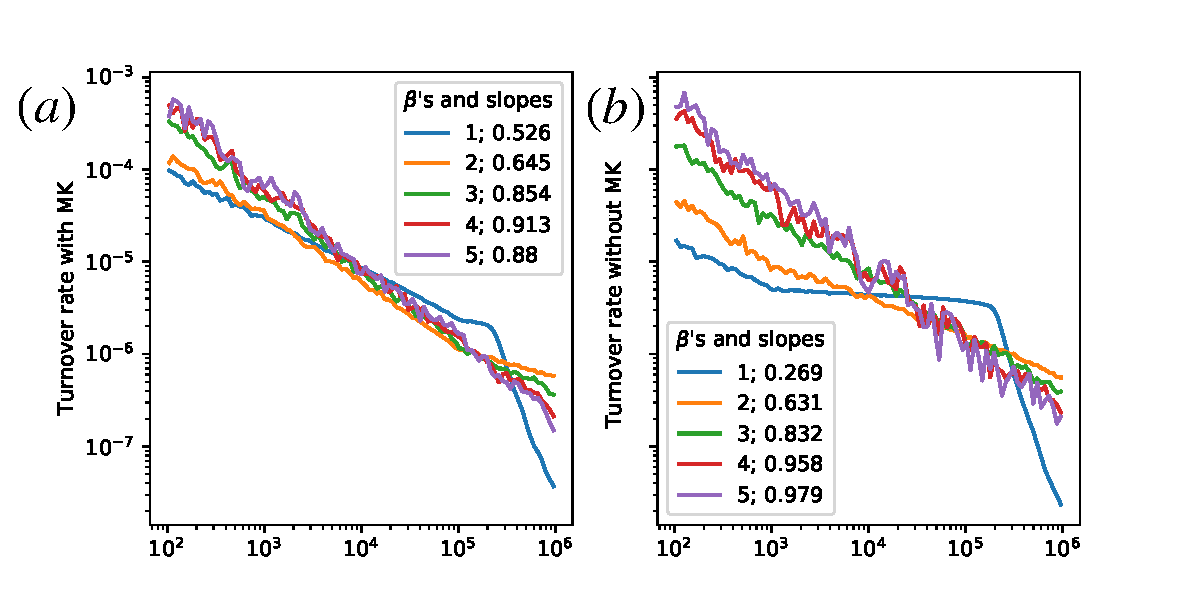
\includegraphics[width = 0.5\textwidth]{sym_suggested_LD/pics/in_one_now_now.pdf}
	\caption{The change rate statistics with and without a memory kernel. The kernel keeps turning over more often. With same $\beta$'s, a kernel-based SYM's decay in turnover rate is smaller. These results validate our prediction that with finite resource, advantages are more likely to be kept.}
	\label{changerate}
\end{figure}

The last property of SYM is the fractality of urban envelop, stately, the length of urban edges vary with the used measurement. Inspired by multi-player interaction in fractal financial market\cite{PhysRevE.65.037106}, we interpret that fractal urban boundary is driven by the competition for land at cities' edges. In SYM, the uncertain competition for space lies in parameter $r$. A larger $r$ indicates larger randomness and brings an extra advantage for minor cities, resulting in a larger fractal dimension. We apply the box counting technique to calculate the fractal dimension of urban envelops, and receive an stable output of $d_f = 1.2\pm 0.05$ with $r = 0.5$, similar to empirical results\cite{batty1992form}. We also find larger $d_f$'s for greater $r$. These results validate our hypothesis that fractal edges coexist with spatial competition. Also, this result also confirms that SYM replicates an urban system.


% 前面加综述
% Despite advances in growth modeling of cities, we still lack a consistent model for both stages of demographic growth and allocation of resources.


\section{Discussion}
% 总结我们这个模型的发现有哪些,为什么我们这个好。
% Future endeavor
% 这两段是新写的。
% In this letter, we have proposed a simple model, spatial preferential growth with finite seeds, to simulate the emergence of cities and reveal the scaling laws as well as how economical dilemma would lead to spatial transitions. We account the emergence and growth of cities by adding and redistributing active population over given area. The model reveals the competition among cities in area and developmental potentials. We 
% This model leads a way in the adaptation of realistic conditions in statistical physical modeling, by regardless of the whole present population within the system, and considering only the active part of them. 
This \emph{Letter} concludes the urban system dynamics in only three key components, and presents fruitful results. The SYM leads a way in the adaptation of realistic conditions in statistical physical modeling, by regardless of the whole present population within the system, and considering only the active part of them. SYM explains existing properties, such as fractality, Zipf's, and Clark's law, where we have both analytical mean-field derivations and bias analysis. More importantly, SYM predicts regional trends in a probabilistic perspective. Due to the simplicity of SYM, we investigate the future phase transition of urban development in great details, and explain dilemmas of the present stage of urbanization through the competitions for systematic resource and space. The assumptions of SYM are well-held if sufficient divergence of meta-population across the world is considered. Simulations of this model can be adjust to heterogeneous geographical circumstances by applying the growing rate on each cell to the product of inherent dynamic $m_{ij}\cdot \beta_2$ and the local characteristic $c_{ij}$ to better suit for realistic conditions.

The memory kernel mechanism leads to a straightforward corollary that the construction of infrastructure drives population's spatial transitions, as only those who are recorded in the kernel are considered as active citizens that attract new-comers to his city. This result provides a bottom-up explanation for transition of urban centers with stochastic spatial shifts of cities' memorized people. It also tells that the economic growth is the basis of growth potentials. Under the circumstances of preferential attraction, if the size of the memory kernel cannot grow fast enough to match with population, the concentration of production will go far from tolerance. 

Taking the productive aspect together in the memory kernel helps to talk about many other properties like the age structure. The stationary age can be calculated as the average time for a new city to emerge is $(\beta_2 N^* + \beta_1 k)^{-1}$, which equals to the average losing age of the whole kernel. This result gives an instruction of the length of workable age in a given social urban system.

% 不足
Although our results are not all analytically proved, we believe it is an essential step to strip out the power of urban dynamics. The model is non-commuting, but the community structure is naturally embedded. For further consideration, we can extend the model by adding links as the volume of exploration and preferential return between cities\cite{WANG2019121921}. The model can further be extended with multi-dimensional memory kernel, allowing one citizen to be introduced if different factors\cite{doi:10.1098/rsif.2019.0564} (i.e., the existing citizens in different dimension of kernel) agree to allow her in the system.



\bibliography{refs.bib}

\end{document}